%Version 3 October 2023
% See section 11 of the User Manual for version history
%
%%%%%%%%%%%%%%%%%%%%%%%%%%%%%%%%%%%%%%%%%%%%%%%%%%%%%%%%%%%%%%%%%%%%%%
%%                                                                 %%
%% Please do not use \input{...} to include other tex files.       %%
%% Submit your LaTeX manuscript as one .tex document.              %%
%%                                                                 %%
%% All additional figures and files should be attached             %%
%% separately and not embedded in the \TeX\ document itself.       %%
%%                                                                 %%
%%%%%%%%%%%%%%%%%%%%%%%%%%%%%%%%%%%%%%%%%%%%%%%%%%%%%%%%%%%%%%%%%%%%%

%%\documentclass[referee,sn-basic]{sn-jnl}% referee option is meant for double line spacing

%%=======================================================%%
%% to print line numbers in the margin use lineno option %%
%%=======================================================%%

%%\documentclass[lineno,sn-basic]{sn-jnl}% Basic Springer Nature Reference Style/Chemistry Reference Style

%%======================================================%%
%% to compile with pdflatex/xelatex use pdflatex option %%
%%======================================================%%

%%\documentclass[pdflatex,sn-basic]{sn-jnl}% Basic Springer Nature Reference Style/Chemistry Reference Style


%%Note: the following reference styles support Namedate and Numbered referencing. By default the style follows the most common style. To switch between the options you can add or remove “Numbered” in the optional parenthesis. 
%%The option is available for: sn-basic.bst, sn-vancouver.bst, sn-chicago.bst%  
 
%%\documentclass[sn-nature]{sn-jnl}% Style for submissions to Nature Portfolio journals
%%\documentclass[sn-basic]{sn-jnl}% Basic Springer Nature Reference Style/Chemistry Reference Style
\documentclass[sn-mathphys-num]{sn-jnl}% Math and Physical Sciences Numbered Reference Style 
%%\documentclass[sn-mathphys-ay]{sn-jnl}% Math and Physical Sciences Author Year Reference Style
%%\documentclass[sn-aps]{sn-jnl}% American Physical Society (APS) Reference Style
%%\documentclass[sn-vancouver,Numbered]{sn-jnl}% Vancouver Reference Style
%%\documentclass[sn-apa]{sn-jnl}% APA Reference Style 
%%\documentclass[sn-chicago]{sn-jnl}% Chicago-based Humanities Reference Style

%%%% Standard Packages
%%<additional latex packages if required can be included here>

\usepackage{graphicx}%
\usepackage{multirow}%
\usepackage{amsmath,amssymb,amsfonts}%
\usepackage{amsthm}%
\usepackage{mathrsfs}%
\usepackage[title]{appendix}%
\usepackage{xcolor}%
\usepackage{textcomp}%
\usepackage{manyfoot}%
\usepackage{booktabs}%
\usepackage{algorithm}%
\usepackage{algorithmicx}%
\usepackage{algpseudocode}%
\usepackage{listings}%
%%%%

%%%%%=============================================================================%%%%
%%%%  Remarks: This template is provided to aid authors with the preparation
%%%%  of original research articles intended for submission to journals published 
%%%%  by Springer Nature. The guidance has been prepared in partnership with 
%%%%  production teams to conform to Springer Nature technical requirements. 
%%%%  Editorial and presentation requirements differ among journal portfolios and 
%%%%  research disciplines. You may find sections in this template are irrelevant 
%%%%  to your work and are empowered to omit any such section if allowed by the 
%%%%  journal you intend to submit to. The submission guidelines and policies 
%%%%  of the journal take precedence. A detailed User Manual is available in the 
%%%%  template package for technical guidance.
%%%%%=============================================================================%%%%

%% as per the requirement new theorem styles can be included as shown below
\theoremstyle{thmstyleone}%
\newtheorem{theorem}{Theorem}%  meant for continuous numbers
%%\newtheorem{theorem}{Theorem}[section]% meant for sectionwise numbers
%% optional argument [theorem] produces theorem numbering sequence instead of independent numbers for Proposition
\newtheorem{proposition}[theorem]{Proposition}% 
%%\newtheorem{proposition}{Proposition}% to get separate numbers for theorem and proposition etc.

\theoremstyle{thmstyletwo}%
\newtheorem{example}{Example}%
\newtheorem{remark}{Remark}%

\theoremstyle{thmstylethree}%
\newtheorem{definition}{Definition}%

\raggedbottom
%%\unnumbered% uncomment this for unnumbered level heads

\begin{document}

\title[Article Title]{Predict Student Performance in Secondary Education Based on Machine Learning Models and Deep Learning Models}



\author*[1]{\fnm{Yanchi} \sur{Liu}}\email{yliu2488@wisc.edu}




%\abstract{The abstract serves both as a general introduction to the topic and as a brief, non-technical summary of the main results and their implications. Authors are advised to check the author instructions for the journal they are submitting to for word limits and if structural elements like subheadings, citations, or equations are permitted.}

%\keywords{keyword1, Keyword2, Keyword3, Keyword4}

%%\pacs[JEL Classification]{D8, H51}

%%\pacs[MSC Classification]{35A01, 65L10, 65L12, 65L20, 65L70}

\maketitle

\section{Introduction}

Academic performance is a complex construct influenced by a myriad of factors. Among these, family characteristics and personal attributes of students are recognized as pivotal determinants. Some literatures explore the interplay between these factors and their impact on educational outcomes. 

Some family characteristics include socioeconomic status, parental education, family structure and stability, and parental involvement. Studies consistently show that students from higher SES backgrounds tend to perform better academically. This is often attributed to greater access to resources, such as quality educational materials and tutoring services \textcolor{blue}{(Entwisle & Alexander, 1992)}. Parental education level is strongly correlated with student performance. Parents with higher education are more likely to engage in activities that foster cognitive development and academic support \textcolor{blue}{(Hill & Tyson, 2009)}. A stable family environment with consistent routines and clear expectations can positively influence academic performance. Conversely, frequent disruptions and instability can lead to stress and reduced focus on studies \textcolor{blue}{(Amato, P. R., 2010.)} Active parental involvement in a child's education, including homework assistance and school engagement, is linked to improved academic outcomes \textcolor{blue}{(Henderson & Mapp, 2002)}. 

Personal characteristics of students include cognitive abilities, motivation and engagement, learning strategies, emotional intelligence, and personal interests and passions. Innate cognitive abilities, including intelligence and memory, are foundational to academic success. However, the extent to which these abilities are nurtured and developed can vary greatly \textcolor{blue}{(Sternberg & Grigorenko, 2002)}. Intrinsic motivation and engagement with learning material are critical. Students who are self-motivated and find learning personally relevant tend to perform better \textcolor{blue}{(Ryan & Deci, 2000)}.  Effective learning strategies, such as organization, time management, and critical thinking, are associated with higher academic performance \textcolor{blue}{(Pintrich, 2004)}. Emotional intelligence, including self-awareness and the ability to manage emotions, can influence academic performance by affecting social interactions and stress management \textcolor{blue}{(Mayer, Salovey, & Caruso, 2008)}. Students who pursue subjects they are passionate about often exhibit higher levels of engagement and performance \textcolor{blue}{(Diemberger, L., 2021)}.

In order to explore the relationships between the student's academic performance and these potential characteristics and build a predictive model for predicting the student's performance based on these characteristics, some machine learning models and deep learning models are applied to the dataset of student performance published on the UCI machine learning repository. 


\section{Description of Dataset}

The dataset used in this report is from the UCI machine learning repository, which collected the student academic performance data in secondary education of two Portuguese schools. The data were obtained by school reports and questionnaires including student grades, demographic, social, school-related features, and parental characteristics. There are two versions of datasets with respect to two subjects: Maths and Portuguese language. In this project, the latter one is chosen for analysis. In addition, there are three grades recorded in this dataset. For simplicity, only the final grade at 3rd period is focused. More details about the dataset can be found at the website, \url{https://archive.ics.uci.edu/dataset/320/student+performance}. 



\section{Exploratory Data Analysis}

The dataset has 643 observations and 33 variables, which is glimpsed Figure 1. The descriptive statistics of some numerical variables are shown in Figure 2. Figure 3 displays the relationship between the outcome variable (final grade) and personal features. There are significant differences in final grades for students of two schools. The average grade of female students is slightly higher than that of male students. The grades of students who are greater than 18 years old are higher than those who are not. With the weekly study time increases, the average grades tend to be higher.  The number of past class failures is a good indicator of grade, with a positive correlation between grades. As for the family features shown in Figure 4, mother's education seems to be positively correlated to students' performance. The parents' job is also a significant factor, where the students whose parents are teachers tend to have a higher grade.


\begin{figure}[h]\label{glimpse_data}
    \centering
    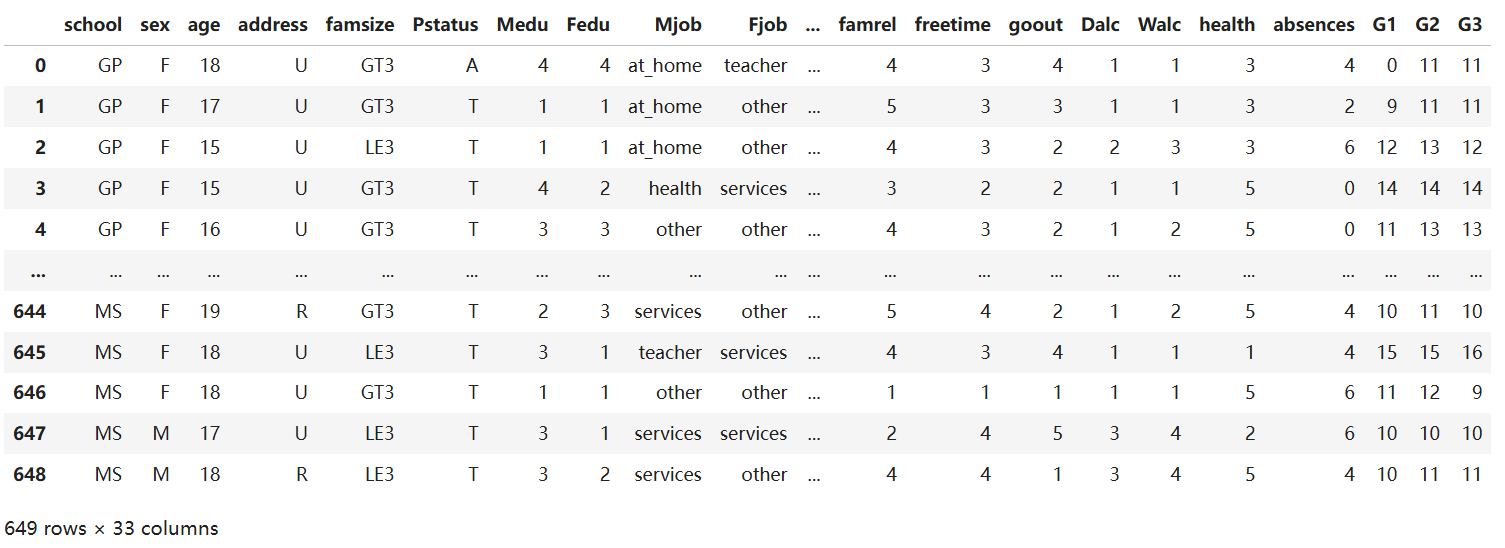
\includegraphics[width=\textwidth]{figure/fig1_glimpse_data.png}
    \caption{The screenshot of the dataset in Jupyter notebook}
\end{figure}

\begin{figure}[h]
    \centering
    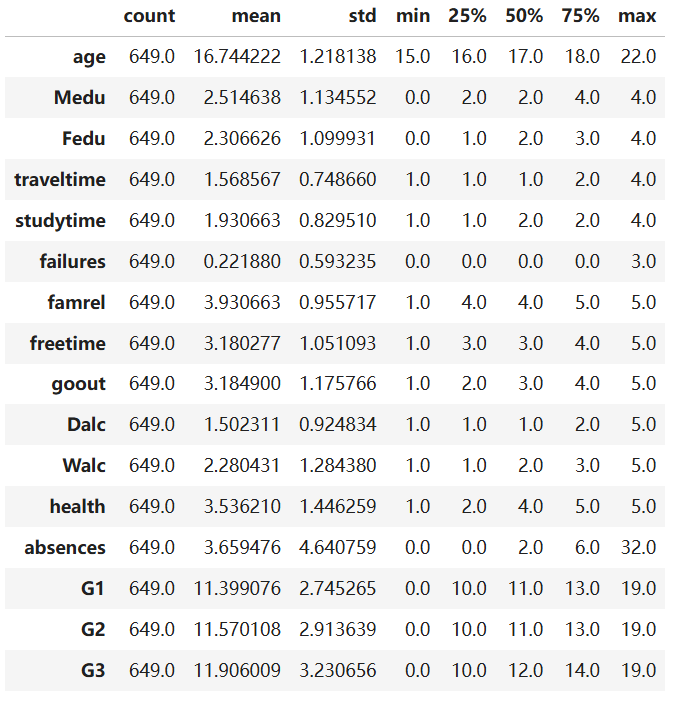
\includegraphics[width=0.7\textwidth]{figure/fig2_description_data.png}
    \caption{The descriptive statistics of some variables in the dataset}
    \label{summary_data}
\end{figure}

\begin{figure}[h]
    \centering
    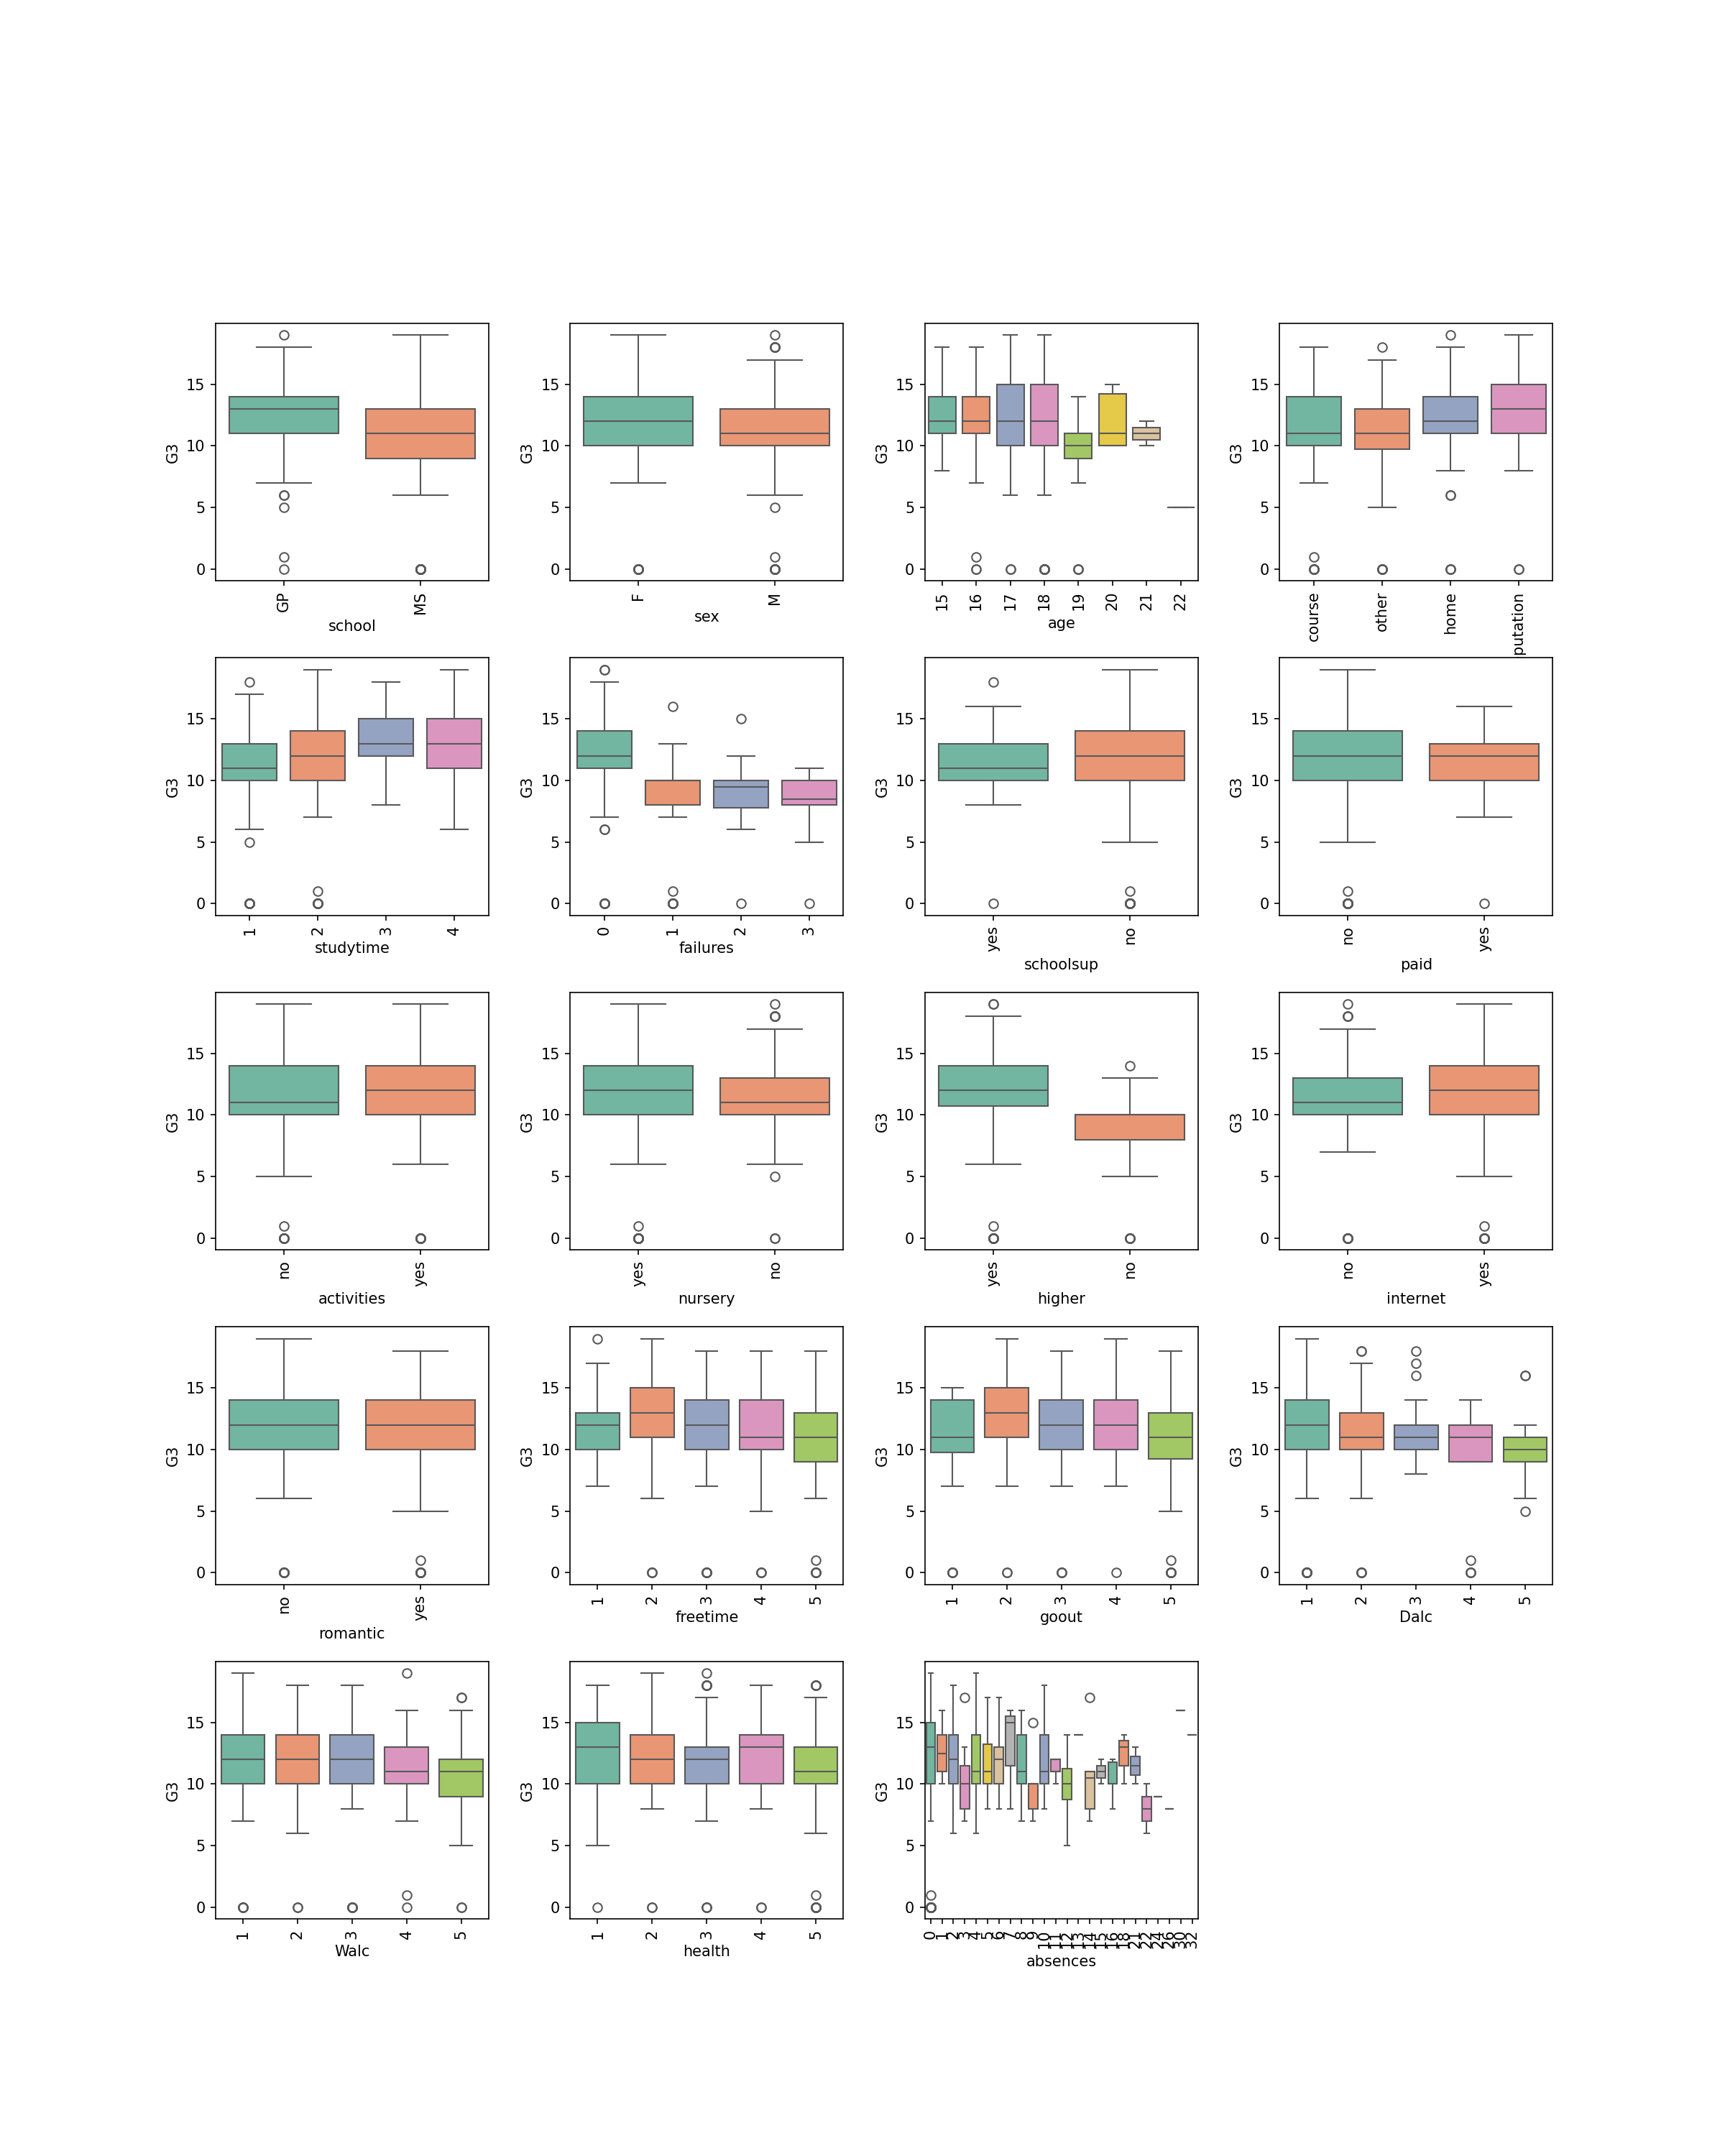
\includegraphics[width=1\textwidth]{figure/fig3_personal_features.png}
    \caption{The boxplots of final grade versus personal features}
\end{figure}

\begin{figure}[h]
    \centering
    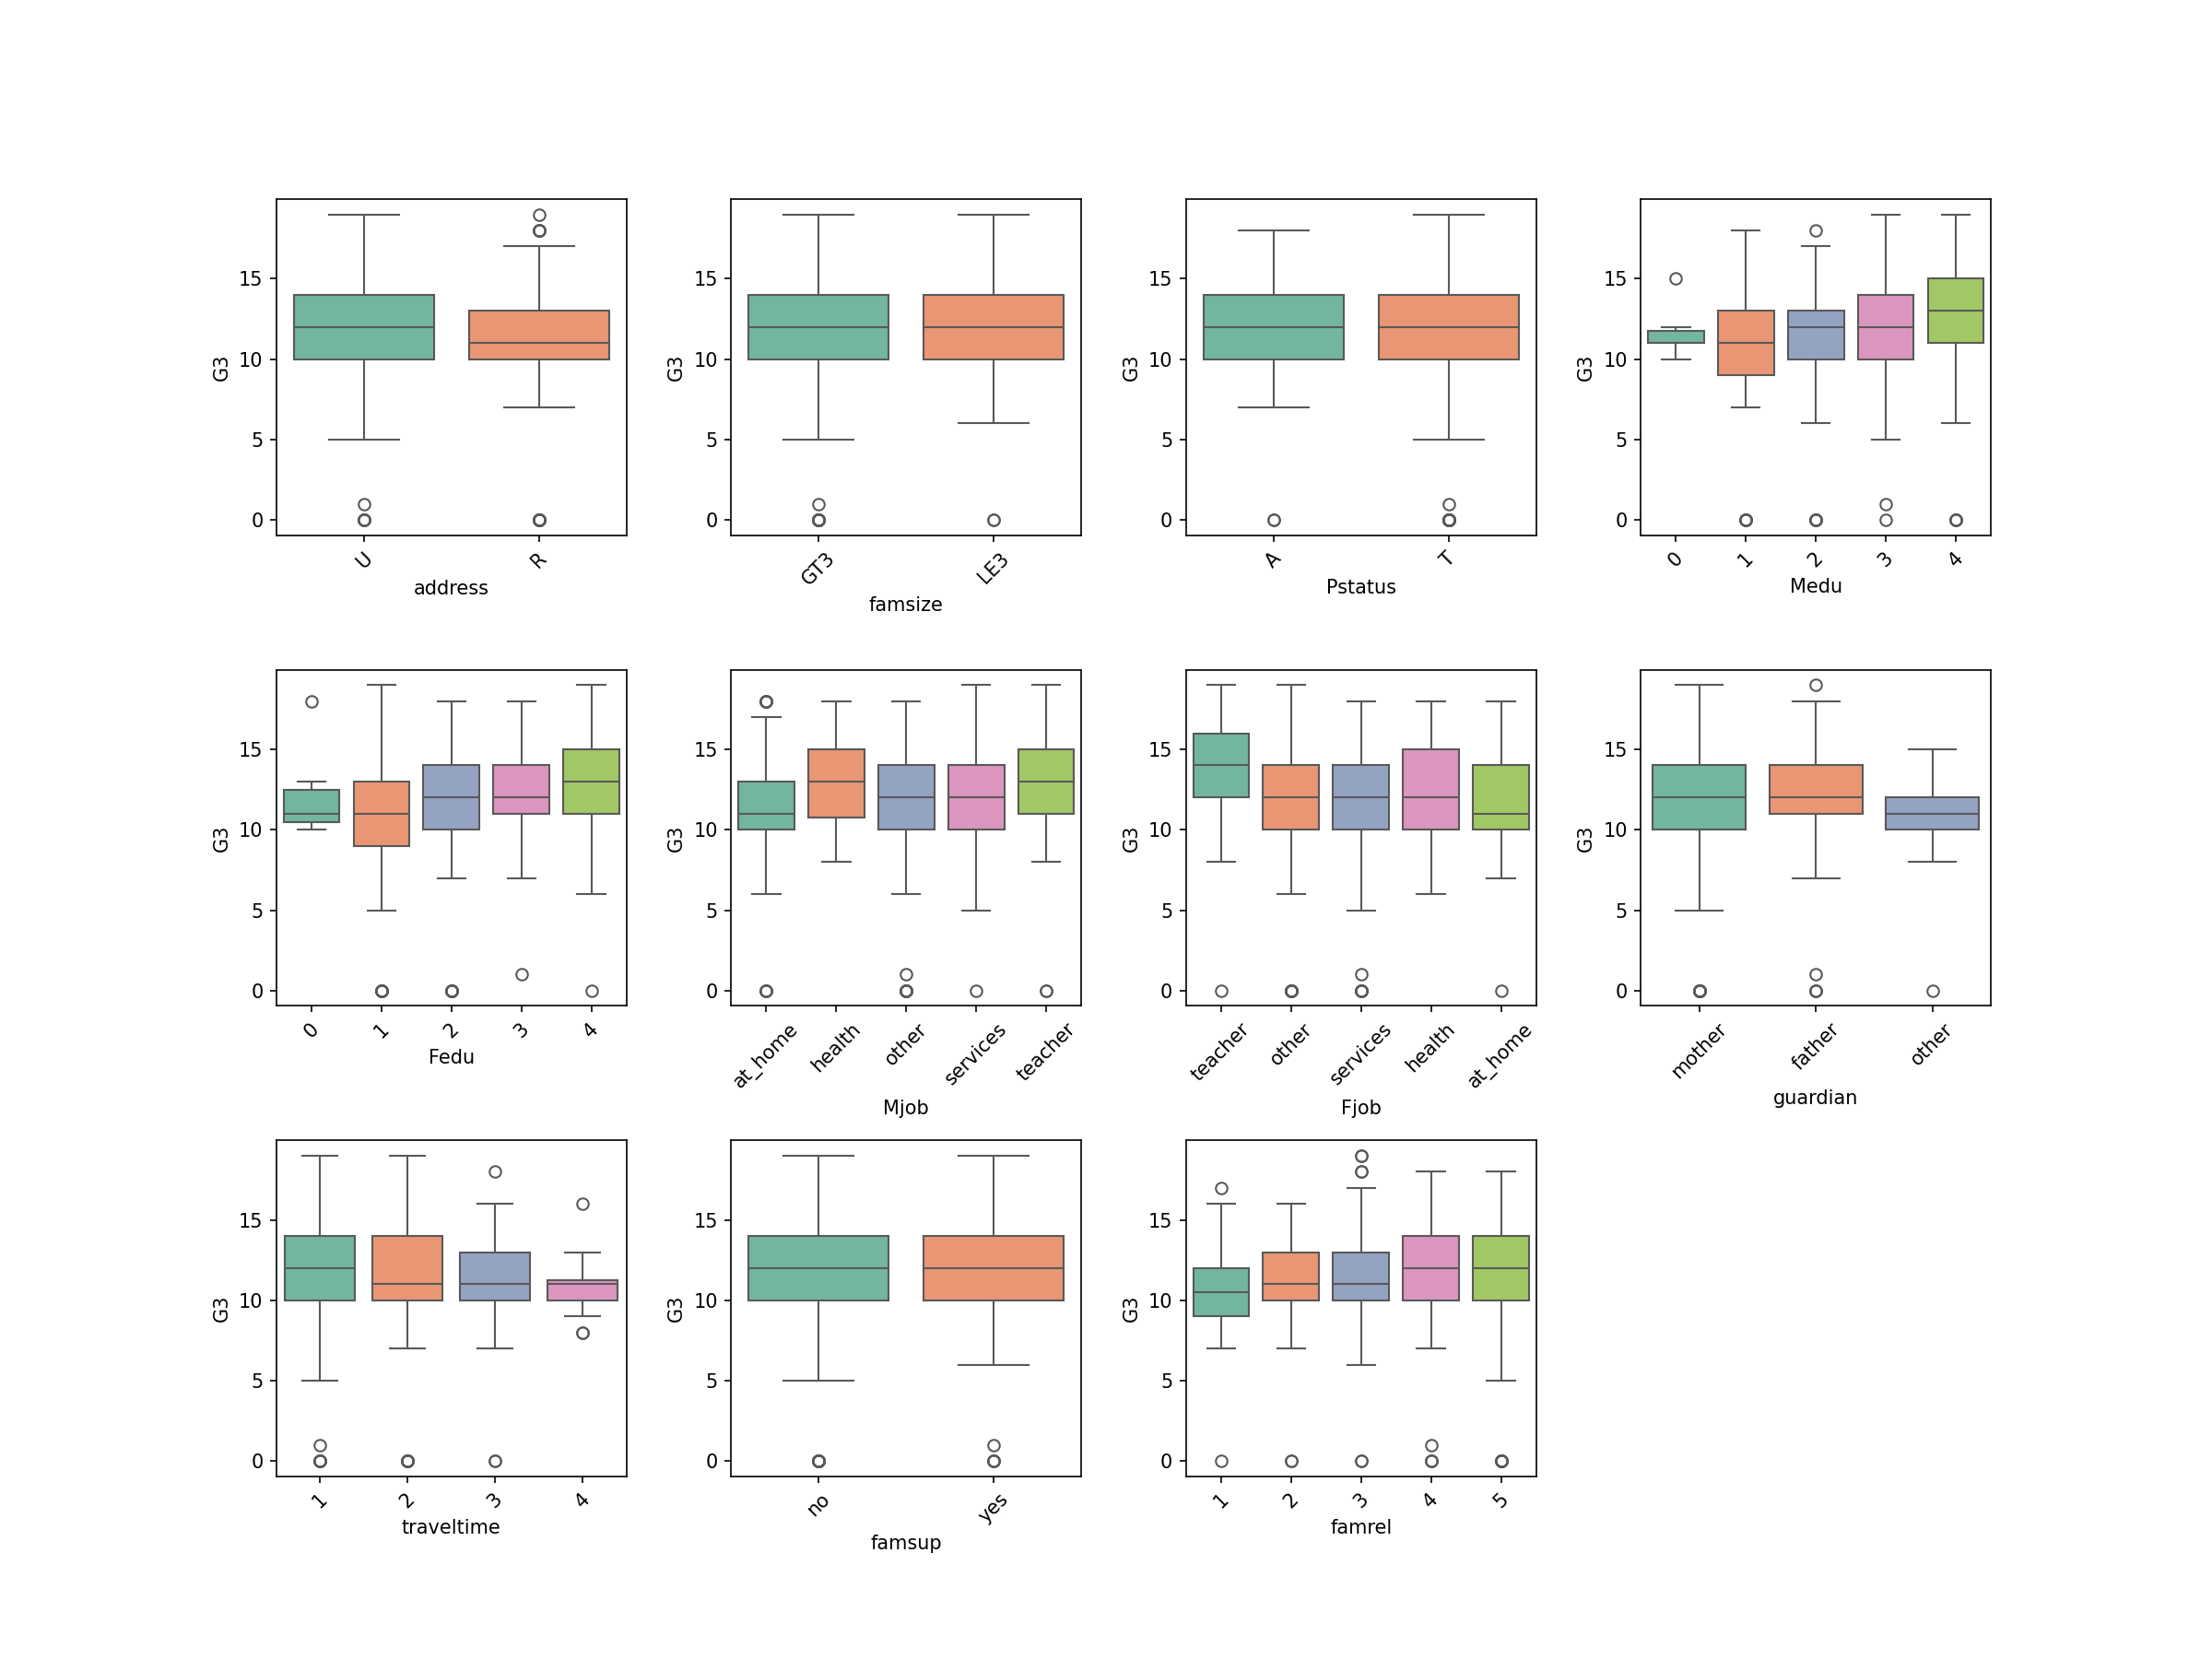
\includegraphics[width=1\textwidth]{figure/fig4_family_features.png}
    \caption{The boxplots of final grade versus family features}
\end{figure}


\clearpage
\section{Models}

\subsection{Regression Tree}

Regression trees \textcolor{blue}{(Breiman et al, 1984, James et al (2013))}  are a non-parametric supervised learning method used for both classification and regression. They create a model in the form of a tree structure, where each internal node denotes a test on an attribute, each branch represents the outcome of the test, and each leaf node holds a numerical value (in regression) or a class label (in classification). The goal is to split the data based on feature values that best separate the target variable, minimizing the variance within each node.

In this report, a regression tree with the maximal depth of 5, and minimal samples in leaves node of 10 is trained. The model performance of this model is summarized in the following table.

\begin{table}[h]
  \centering
  \caption{The performance of the regression tree }
  \begin{tabular}{c|c|c}
  \hline
   Index  &  Training  & Test\\
   \hline
   MSE  &  2.45555  & 2.96739 \\
   \hline
   MAE  &  1.88155  & 2.28019\\
   \hline
   $R^2$  &  0.42715  & 0.09704 \\
   \hline
  \end{tabular}
\end{table}

\begin{figure}[h]
    \centering
    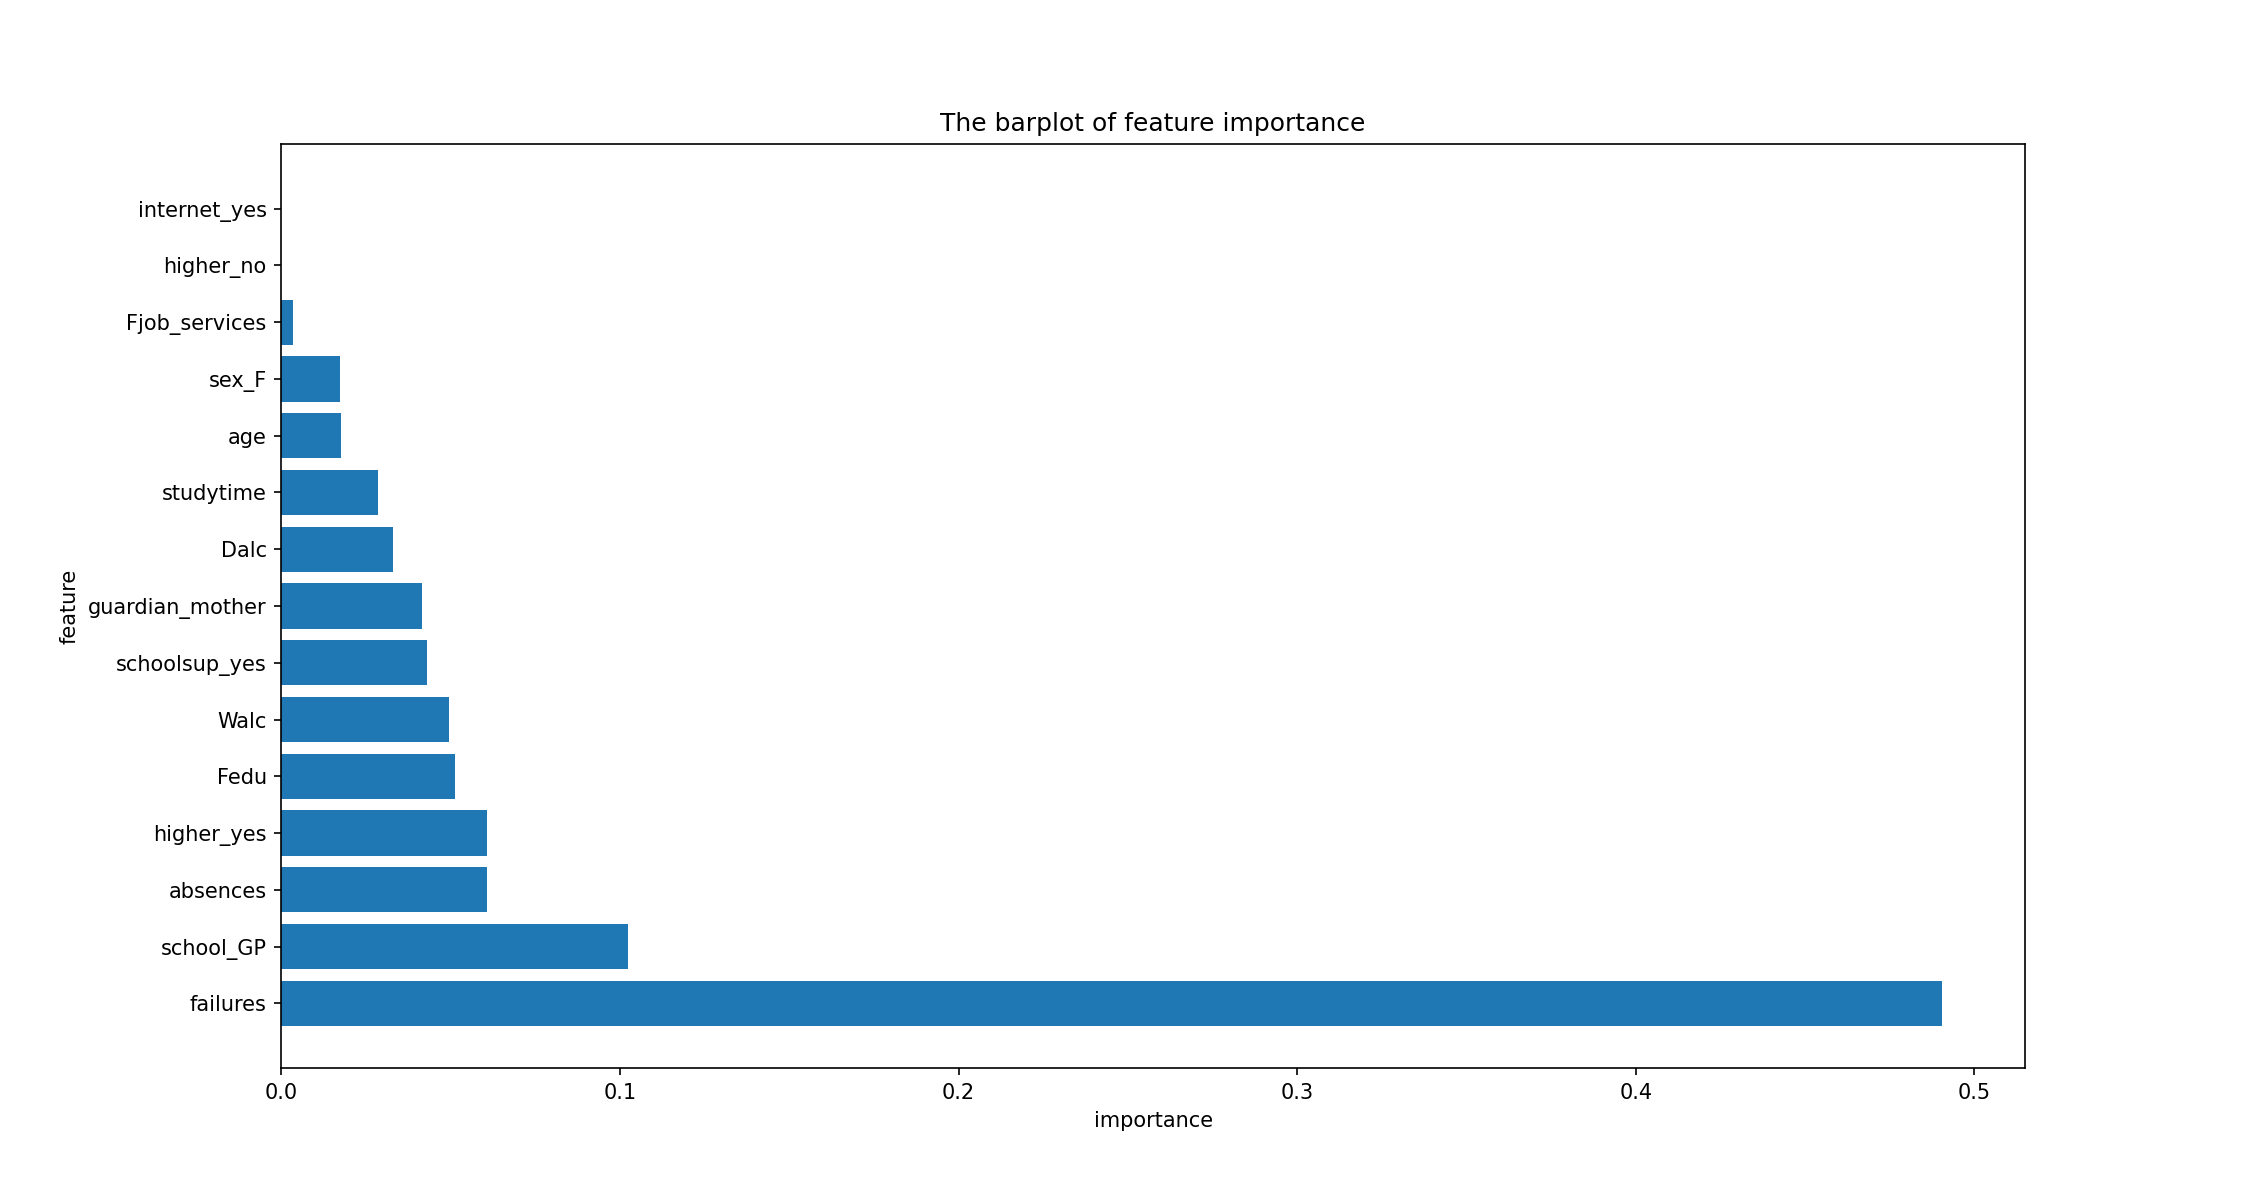
\includegraphics[width=\textwidth]{figure/feature_importance_regression_tree.png}
    \caption{The bar plot of feature importance obtained by regression tree}
\end{figure}

The bar plot of feature importance demonstrates that the number of past class failures, the school, and the number of school absences are the top three important features. It shows that personal features are more influential on students' academic performance. As for parental features, the guardian of the student and the father's job are significantot factors. The performance of XGBOOST is greater than that of the regression tree, showing the power of ensemble learning. The feature importance results are similar with that of the regression tree.







\subsection{XGBOOST}


XGBoost \textcolor{blue}{(Chen et al, 2016)} is an optimized distributed gradient boosting system designed to be highly efficient, flexible, and portable. It implements machine learning algorithms under the gradient boosting framework. XGBoost provides a parallel tree boosting that solve many data-science problems in a fast and accurate way. It is widely used for machine learning competitions and real-world applications due to its speed and performance.


\begin{table}[h]
  \centering
  \caption{The performance of XGBOOST}
  \begin{tabular}{c|c|c}
  \hline
   Index  &  Training  & Test\\
   \hline
   MSE  &  0.00265  & 2.75889\\
   \hline
   MAE  &  0.00136  & 2.15162\\
   \hline
   $R^2$  &  1  & 0.21947 \\
   \hline
  \end{tabular}
\end{table}

\begin{figure}[h]
    \centering
    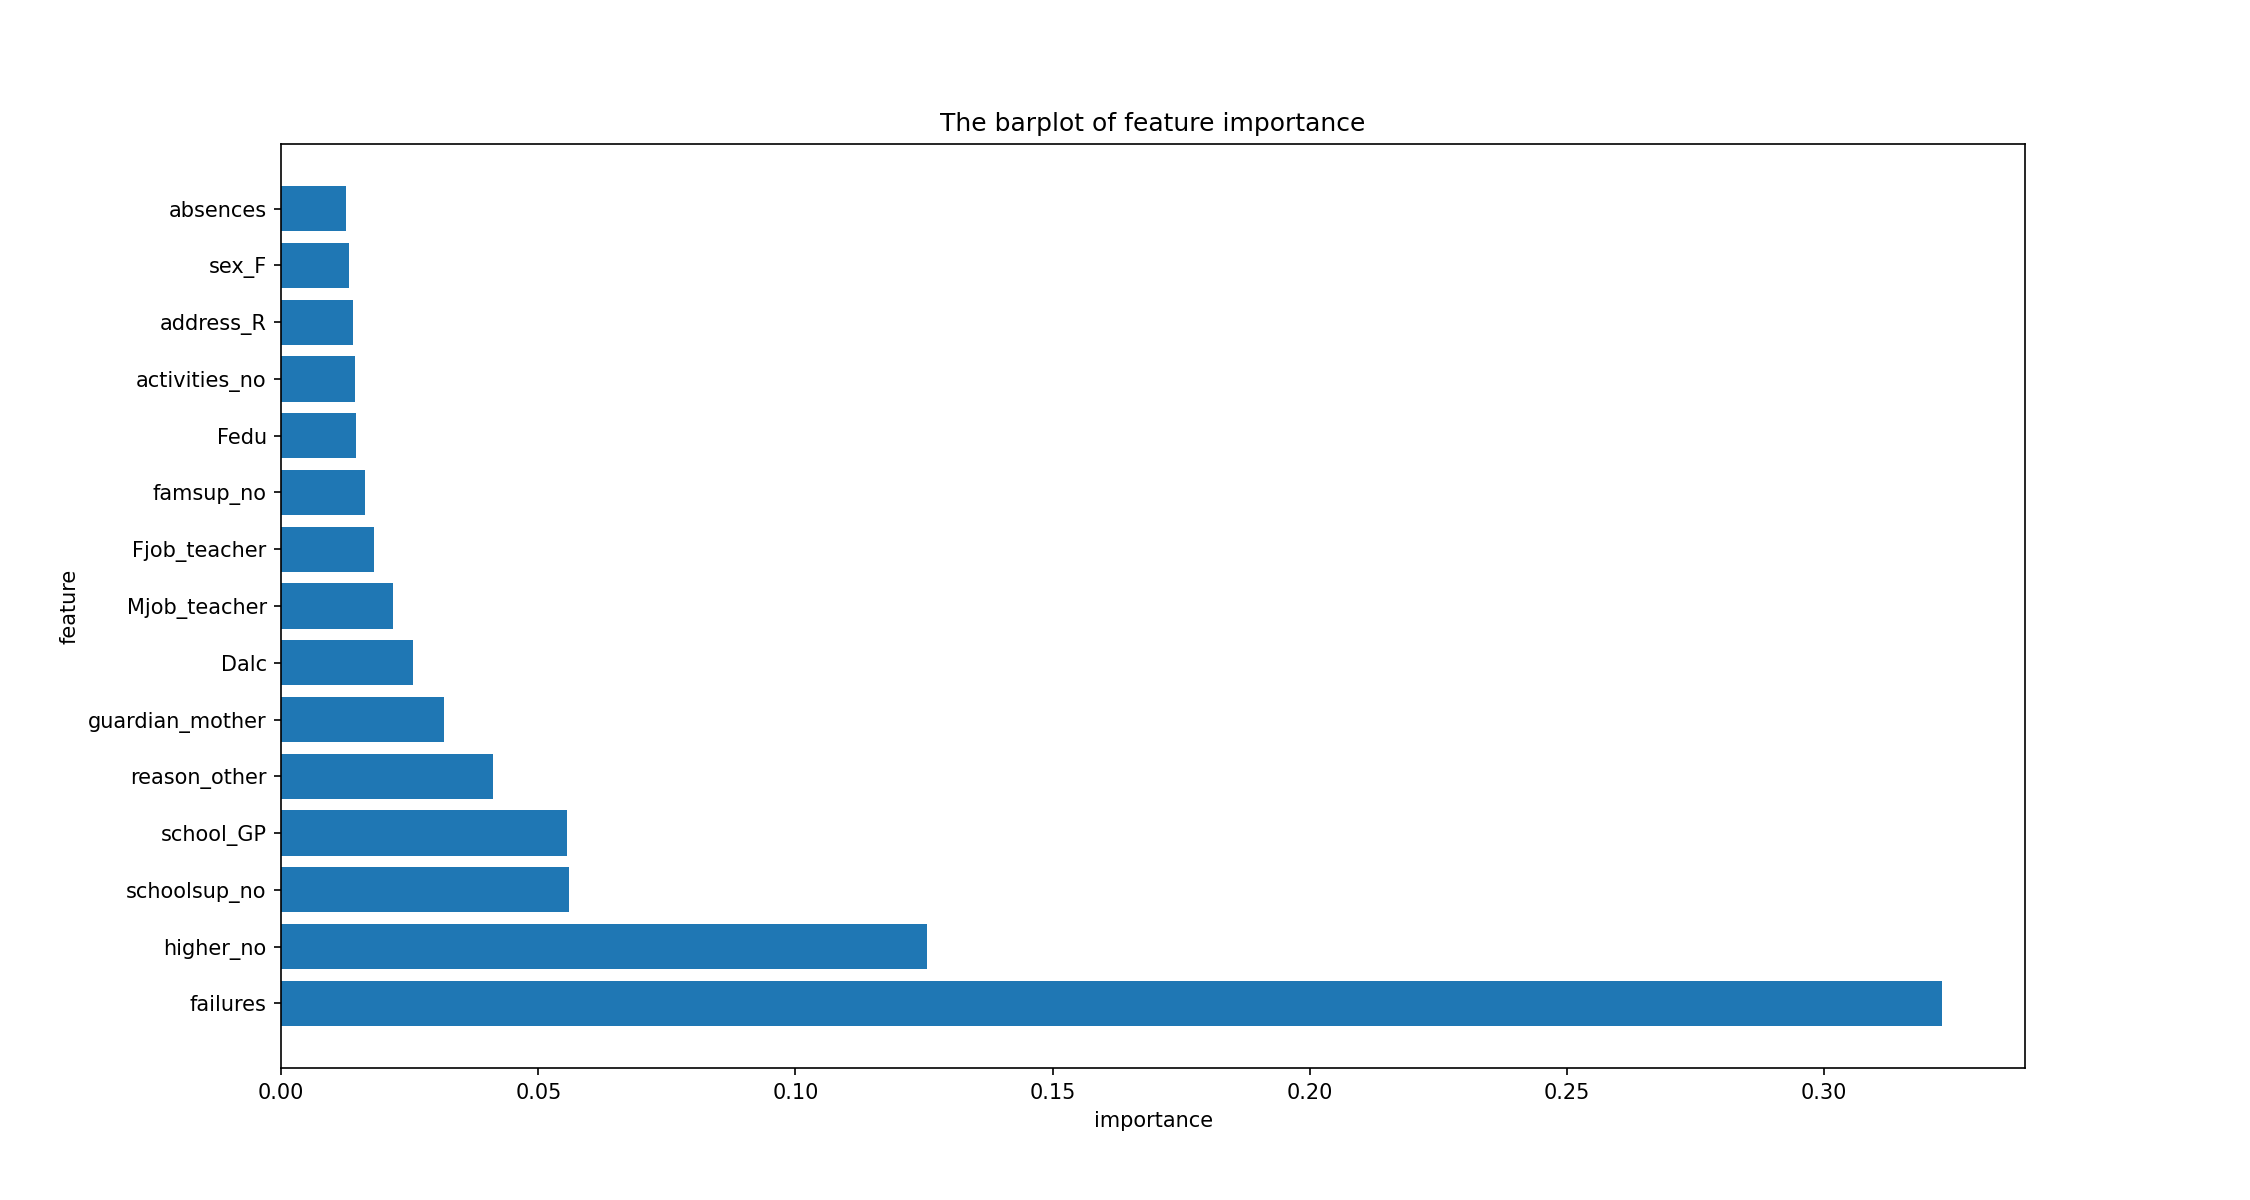
\includegraphics[width=\textwidth]{figure/feature_importance_xgboost.png}
    \caption{The bar plot of feature importance obtained by regression tree}
\end{figure}


\subsection{MLP}

Multilayer Perceptrons (MLPs) are a class of feedforward artificial neural networks that consist of an input layer, one or more hidden layers, and an output layer \textcolor{blue}{(Goodfellow, 2016)}. They use a supervised learning technique called backpropagation for training, where the error is propagated backward to update the weights. MLPs can model complex relationships between inputs and outputs and are widely used for classification and regression tasks. Based on the following table, it can be found that the performance of MLP is not better than XGBOOST.

\begin{table}[h]
  \centering
  \caption{The performance of MLP}
  \begin{tabular}{c|c|c}
  \hline
   Index  &  Training  & Test\\
   \hline
   MSE  &  1.87993  & 2.92744\\
   \hline
   MAE  & 1.35962  & 2.19092\\
   \hline
   $R^2$  &  0.66424  & 0.12119 \\
   \hline
  \end{tabular}
\end{table}



\subsection{DNN}


Deep Neural Networks (DNNs) \textcolor{blue}{(Goodfellow, 2016)} are a class of artificial neural networks with multiple layers of interconnected nodes, beyond the simple perceptron structure. They leverage the power of deep learning to learn hierarchical feature representations from data. DNNs have revolutionized fields like computer vision and natural language processing due to their ability to capture complex patterns and relationships within large datasets.

The loss function used in this project is MSE. The training loss is 0.0032, while the test loss is 
12.6576. The trace plot of training loss for DNN model is given in the following figure.
\begin{figure}[H]
    \centering
    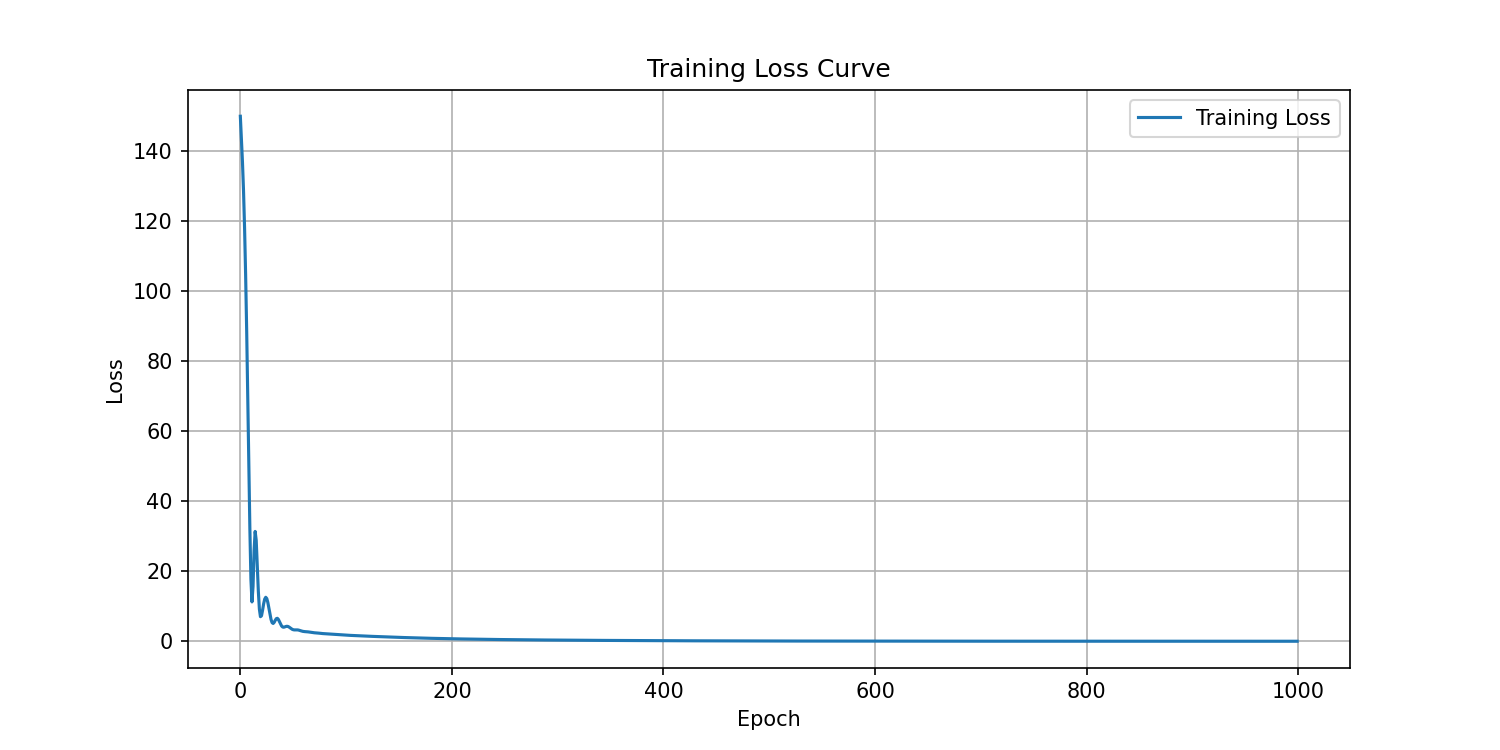
\includegraphics[width=\textwidth]{figure/DNN_loss.png}
    \caption{The training loss plot of DNN}
\end{figure}



\subsection{CNN}

Convolutional Neural Networks (CNNs) are a type of deep learning model designed for processing data with a grid-like topology, such as images \textcolor{blue}{(Krizhevsky, 2012; Simonyan, 2014)}. They utilize convolutional layers to automatically and adaptively learn spatial hierarchies of features from input data. CNNs have achieved state-of-the-art performance in image recognition, video analysis, and other visual computing tasks.

The loss function used in this project is MSE. The training loss is  5.4281, while the test loss is 
8.4673. The trace plot of training loss for CNN model is given in the following figure.
\begin{figure}[H]
    \centering
    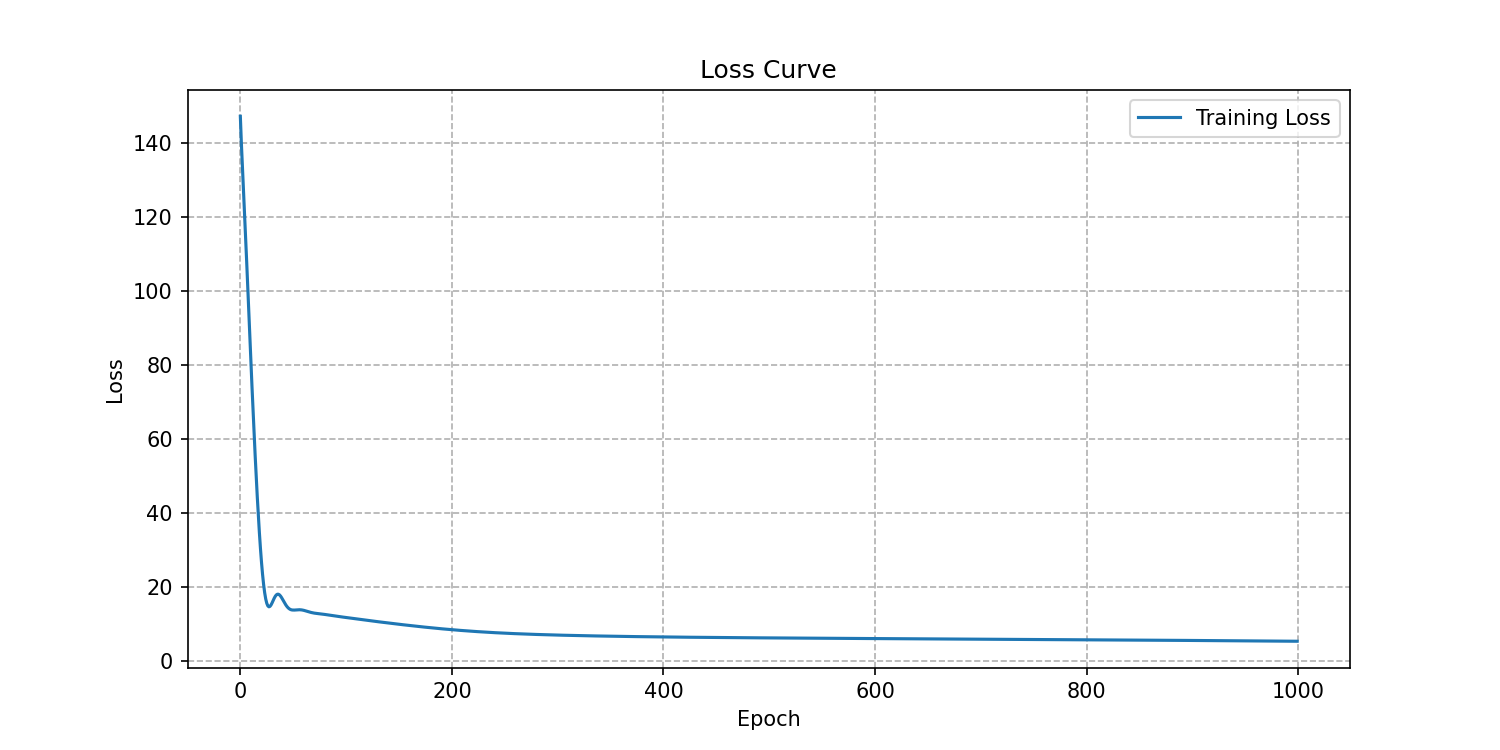
\includegraphics[width=\textwidth]{figure/CNN_loss.png}
    \caption{The training loss plot of CNN}
\end{figure}


\section{Discussion and Conclusion}

In this project, some machine learning methods and deep learning methods are employed to explore the dataset for students' academic performance. Compared to deep learning models, two tree-based machine learning models are more interpretable, where the model results show that personal characteristics are more significant and influential for students' exam grades. As for parental features, the guardian and father's jobs are significant factors for students' performance.  These deep learning models, MLP, DNN and CNN, are used for predicting the students' grades based on the characteristics. But these deep learning models do not outperform machine learning models. It may be due to reasons such as limited data availability, data sizes, overfitting when not enough regularization is applied, and the effectiveness of well-crafted features in traditional models. 


\clearpage
\backmatter

\bmhead{Supplementary Material}

The data, python code in the Jupyter notbook and Latex source code for this project can be found at my Github repository \url{https://github.com/Yc-L722/psych755_project.git}.





\section*{References}

\noindent \url{https://archive.ics.uci.edu/dataset/320/student+performance}

\vspace{1em}

%\noindent  %\url{https://www.semanticscholar.org/paper/Using-data-mining-to-predict-secondary-school-Cortez-Silva/61d468d5254730bbecf822c6b60d7d6595d9889c}

\vspace{1em}

\noindent Entwisle, D. R., & Alexander, K. L. (1992). Summer setback: Race, poverty, school composition, and mathematics achievement in the first two years of school. American Sociological Review, 72-84.


\noindent Hill, N. E., & Tyson, D. F. (2009). Parental involvement in middle school: a meta-analytic assessment of the strategies that promote achievement. Developmental psychology, 45(3), 740.

\vspace{1em}

\noindent Amato, P. R. (2010). The marriage-go-round: The state of marriage and the family in America Today.

\vspace{1em}

\noindent Henderson, A. T., & Mapp, K. L. (2002). A New Wave of Evidence: The Impact of School, Family, and Community Connections on Student Achievement. Annual Synthesis, 2002.

\vspace{1em}

\noindent Sternberg, R. J., & Grigorenko, E. L. (2002). Dynamic testing: The nature and measurement of learning potential. Cambridge university press.

\vspace{1em}

\noindent Ryan, R. M., & Deci, E. L. (2000). Self-determination theory and the facilitation of intrinsic motivation, social development, and well-being. American psychologist, 55(1), 68.

\vspace{1em}

\noindent Pintrich, P. R. (2004). A conceptual framework for assessing motivation and self-regulated learning in college students. Educational psychology review, 16, 385-407.

\vspace{1em}

\noindent Mayer, J. D., Salovey, P., & Caruso, D. R. (2008). Emotional intelligence: New ability or eclectic traits?. American psychologist, 63(6), 503.

\vspace{1em}

\noindent Diemberger, L. (2021). Mindset Psychology of Success. Lorenz Diemberger.


\vspace{1em}

\noindent  Breiman, L., Friedman, J. H., Olshen, R. A., & Stone, C. J. (1984). Classification and Regression Trees. Wadsworth & Brooks/Cole Advanced Books & Software.


\vspace{1em}

\noindent James, G., Witten, D., Hastie, T., & Tibshirani, R. (2013). An Introduction to Statistical Learning: with Applications in R. Springer.

\vspace{1em}

\noindent Chen, T., & Guestrin, C. (2016). XGBoost: A Scalable Tree Boosting System. In Proceedings of the 22nd ACM SIGKDD International Conference on Knowledge Discovery and Data Mining (KDD).

\vspace{1em}

\noindent  Goodfellow, I., Bengio, Y., & Courville, A. (2016). "Deep Learning." MIT Press.

\vspace{1em}

\noindent Krizhevsky, A., Sutskever, I., & Hinton, G. E. (2012). "ImageNet classification with deep convolutional neural networks." Advances in Neural Information Processing Systems, 25, 1097-1105.

\vspace{1em}

\noindent Simonyan, K., & Zisserman, A. (2014). "Very deep convolutional networks for large-scale image recognition." arXiv preprint arXiv:1409.1556.

\end{document}
